%%%%%%%%%%%%%%%%%%%%%%%%%%%%%%%%%%%%%%%%%
% Beamer Presentation
% LaTeX Template
% Version 2.0 (March 8, 2022)
%
% This template originates from:
% https://www.LaTeXTemplates.com
%
% Author:
% Vel (vel@latextemplates.com)
%
% License:
% CC BY-NC-SA 4.0 (https://creativecommons.org/licenses/by-nc-sa/4.0/)
%
%%%%%%%%%%%%%%%%%%%%%%%%%%%%%%%%%%%%%%%%%

%----------------------------------------------------------------------------------------
%	PACKAGES AND OTHER DOCUMENT CONFIGURATIONS
%----------------------------------------------------------------------------------------

\documentclass[
	11pt,]{beamer}

\graphicspath{{Images/}{./}} 

\usepackage{booktabs} 
\usepackage[T1]{fontenc}
\usepackage[polish]{babel}
\usepackage[utf8]{inputenc}

%----------------------------------------------------------------------------------------
%	SELECT LAYOUT THEME
%----------------------------------------------------------------------------------------

% Beamer comes with a number of default layout themes which change the colors and layouts of slides. Below is a list of all themes available, uncomment each in turn to see what they look like.

%\usetheme{default}
%\usetheme{AnnArbor}
%\usetheme{Antibes}
%\usetheme{Bergen}
%\usetheme{Berkeley}
%\usetheme{Berlin}
%\usetheme{Boadilla}
%\usetheme{CambridgeUS}
%\usetheme{Copenhagen}
%\usetheme{Darmstadt}
%\usetheme{Dresden}
%\usetheme{Frankfurt}
%\usetheme{Goettingen}
%\usetheme{Hannover}
%\usetheme{Ilmenau}
%\usetheme{JuanLesPins}
%\usetheme{Luebeck}
\usetheme{Madrid}
%\usetheme{Malmoe}
%\usetheme{Marburg}
%\usetheme{Montpellier}
%\usetheme{PaloAlto}
%\usetheme{Pittsburgh}
%\usetheme{Rochester}
%\usetheme{Singapore}
%\usetheme{Szeged}
%\usetheme{Warsaw}

%----------------------------------------------------------------------------------------
%	SELECT COLOR THEME
%----------------------------------------------------------------------------------------

% Beamer comes with a number of color themes that can be applied to any layout theme to change its colors. Uncomment each of these in turn to see how they change the colors of your selected layout theme.

%\usecolortheme{albatross}
%\usecolortheme{beaver}
%\usecolortheme{beetle}
%\usecolortheme{crane}
\usecolortheme{dolphin}
%\usecolortheme{dove}
%\usecolortheme{fly}
%\usecolortheme{lily}
%\usecolortheme{monarca}
%\usecolortheme{seagull}
%\usecolortheme{seahorse}
%\usecolortheme{spruce}
%\usecolortheme{whale}
%\usecolortheme{wolverine}

%----------------------------------------------------------------------------------------
%	SELECT FONT THEME & FONTS
%----------------------------------------------------------------------------------------

% Beamer comes with several font themes to easily change the fonts used in various parts of the presentation. Review the comments beside each one to decide if you would like to use it. Note that additional options can be specified for several of these font themes, consult the beamer documentation for more information.

\usefonttheme{default} % Typeset using the default sans serif font
%\usefonttheme{serif} % Typeset using the default serif font (make sure a sans font isn't being set as the default font if you use this option!)
%\usefonttheme{structurebold} % Typeset important structure text (titles, headlines, footlines, sidebar, etc) in bold
%\usefonttheme{structureitalicserif} % Typeset important structure text (titles, headlines, footlines, sidebar, etc) in italic serif
%\usefonttheme{structuresmallcapsserif} % Typeset important structure text (titles, headlines, footlines, sidebar, etc) in small caps serif

%------------------------------------------------

%\usepackage{mathptmx} % Use the Times font for serif text
\usepackage{palatino} % Use the Palatino font for serif text
\usepackage{svg}
%\usepackage{helvet} % Use the Helvetica font for sans serif text
\usepackage[default]{opensans} % Use the Open Sans font for sans serif text
%\usepackage[default]{FiraSans} % Use the Fira Sans font for sans serif text
%\usepackage[default]{lato} % Use the Lato font for sans serif text

%----------------------------------------------------------------------------------------
%	SELECT INNER THEME
%----------------------------------------------------------------------------------------

% Inner themes change the styling of internal slide elements, for example: bullet points, blocks, bibliography entries, title pages, theorems, etc. Uncomment each theme in turn to see what changes it makes to your presentation.

%\useinnertheme{default}
\useinnertheme{circles}
%\useinnertheme{rectangles}
%\useinnertheme{rounded}
%\useinnertheme{inmargin}

%----------------------------------------------------------------------------------------
%	SELECT OUTER THEME
%----------------------------------------------------------------------------------------

% Outer themes change the overall layout of slides, such as: header and footer lines, sidebars and slide titles. Uncomment each theme in turn to see what changes it makes to your presentation.

%\useoutertheme{default}
%\useoutertheme{infolines}
%\useoutertheme{miniframes}
%\useoutertheme{smoothbars}
%\useoutertheme{sidebar}
%\useoutertheme{split}
%\useoutertheme{shadow}
%\useoutertheme{tree}
%\useoutertheme{smoothtree}

%\setbeamertemplate{footline} % Uncomment this line to remove the footer line in all slides
%\setbeamertemplate{footline}[page number] % Uncomment this line to replace the footer line in all slides with a simple slide count

%\setbeamertemplate{navigation symbols}{} % Uncomment this line to remove the navigation symbols from the bottom of all slides

%----------------------------------------------------------------------------------------
%	PRESENTATION INFORMATION
%----------------------------------------------------------------------------------------

\title[VecEdit]{Edytor grafiki wektorowej} \subtitle{} 

\author[]{Adam Rogowski \and Szymon Sawoń \and Bartosz Siemaszkiewicz} 

\date[16 grudnia 2024]{Zaawansowane techniki programistyczne \\ 16 grudnia 2024} 

%----------------------------------------------------------------------------------------

\begin{document}

%----------------------------------------------------------------------------------------
%	TITLE SLIDE
%----------------------------------------------------------------------------------------

\begin{frame}
	\titlepage 
\end{frame}

\begin{frame}
	\frametitle{Spis treści}
	\tableofcontents 
\end{frame}

%----------------------------------------------------------------------------------------
%	PRESENTATION BODY SLIDES
%----------------------------------------------------------------------------------------

\section{Opis projektu} 

\begin{frame}
	\frametitle{Opis projektu}
	
	Aplikacja pozwala na tworzenie, edycję i organizację grafik wektorowych za pomocą prostych narzędzi. Użytkownik może
	\begin{itemize}
		\item rysować podstawowe kształty (np. linie, prostokąty, elipsy, wielokąty),
		\item modyfikować ich właściwości (kolor, obrys, przezroczystość),
		\item przesuwać i skalować obiekty,
		\item grupować je i zarządzać warstwami (w tym ukrywać je, blokować lub zmieniać ich kolejność).
		\item zaznaczać pojedyncze obiekty lub obszary, wycinać je i wklejać, cofać i ponawiać zmiany, 
		\item wyrównywać obiekty do siatki lub względem siebie. 

	\end{itemize}

Aplikacja umożliwia zapisywanie projektów w formacie wektorowym (np. SVG) oraz eksportowanie ich do popularnych formatów graficznych (np. PNG, JPEG).

	\end{frame}

%------------------------------------------------

\section{Diagram klas}

\begin{frame}
	\frametitle{Diagram klas}
	
	\begin{figure}
		\includegraphics[height=0.7\textheight]{figures/class_diagram.pdf}
	\end{figure}
\end{frame}

%------------------------------------------------

\section{Wzorce projektowe}

\subsection{Kompozyt}

\begin{frame}
	\frametitle{Kompozyt}
	
	\begin{figure}
		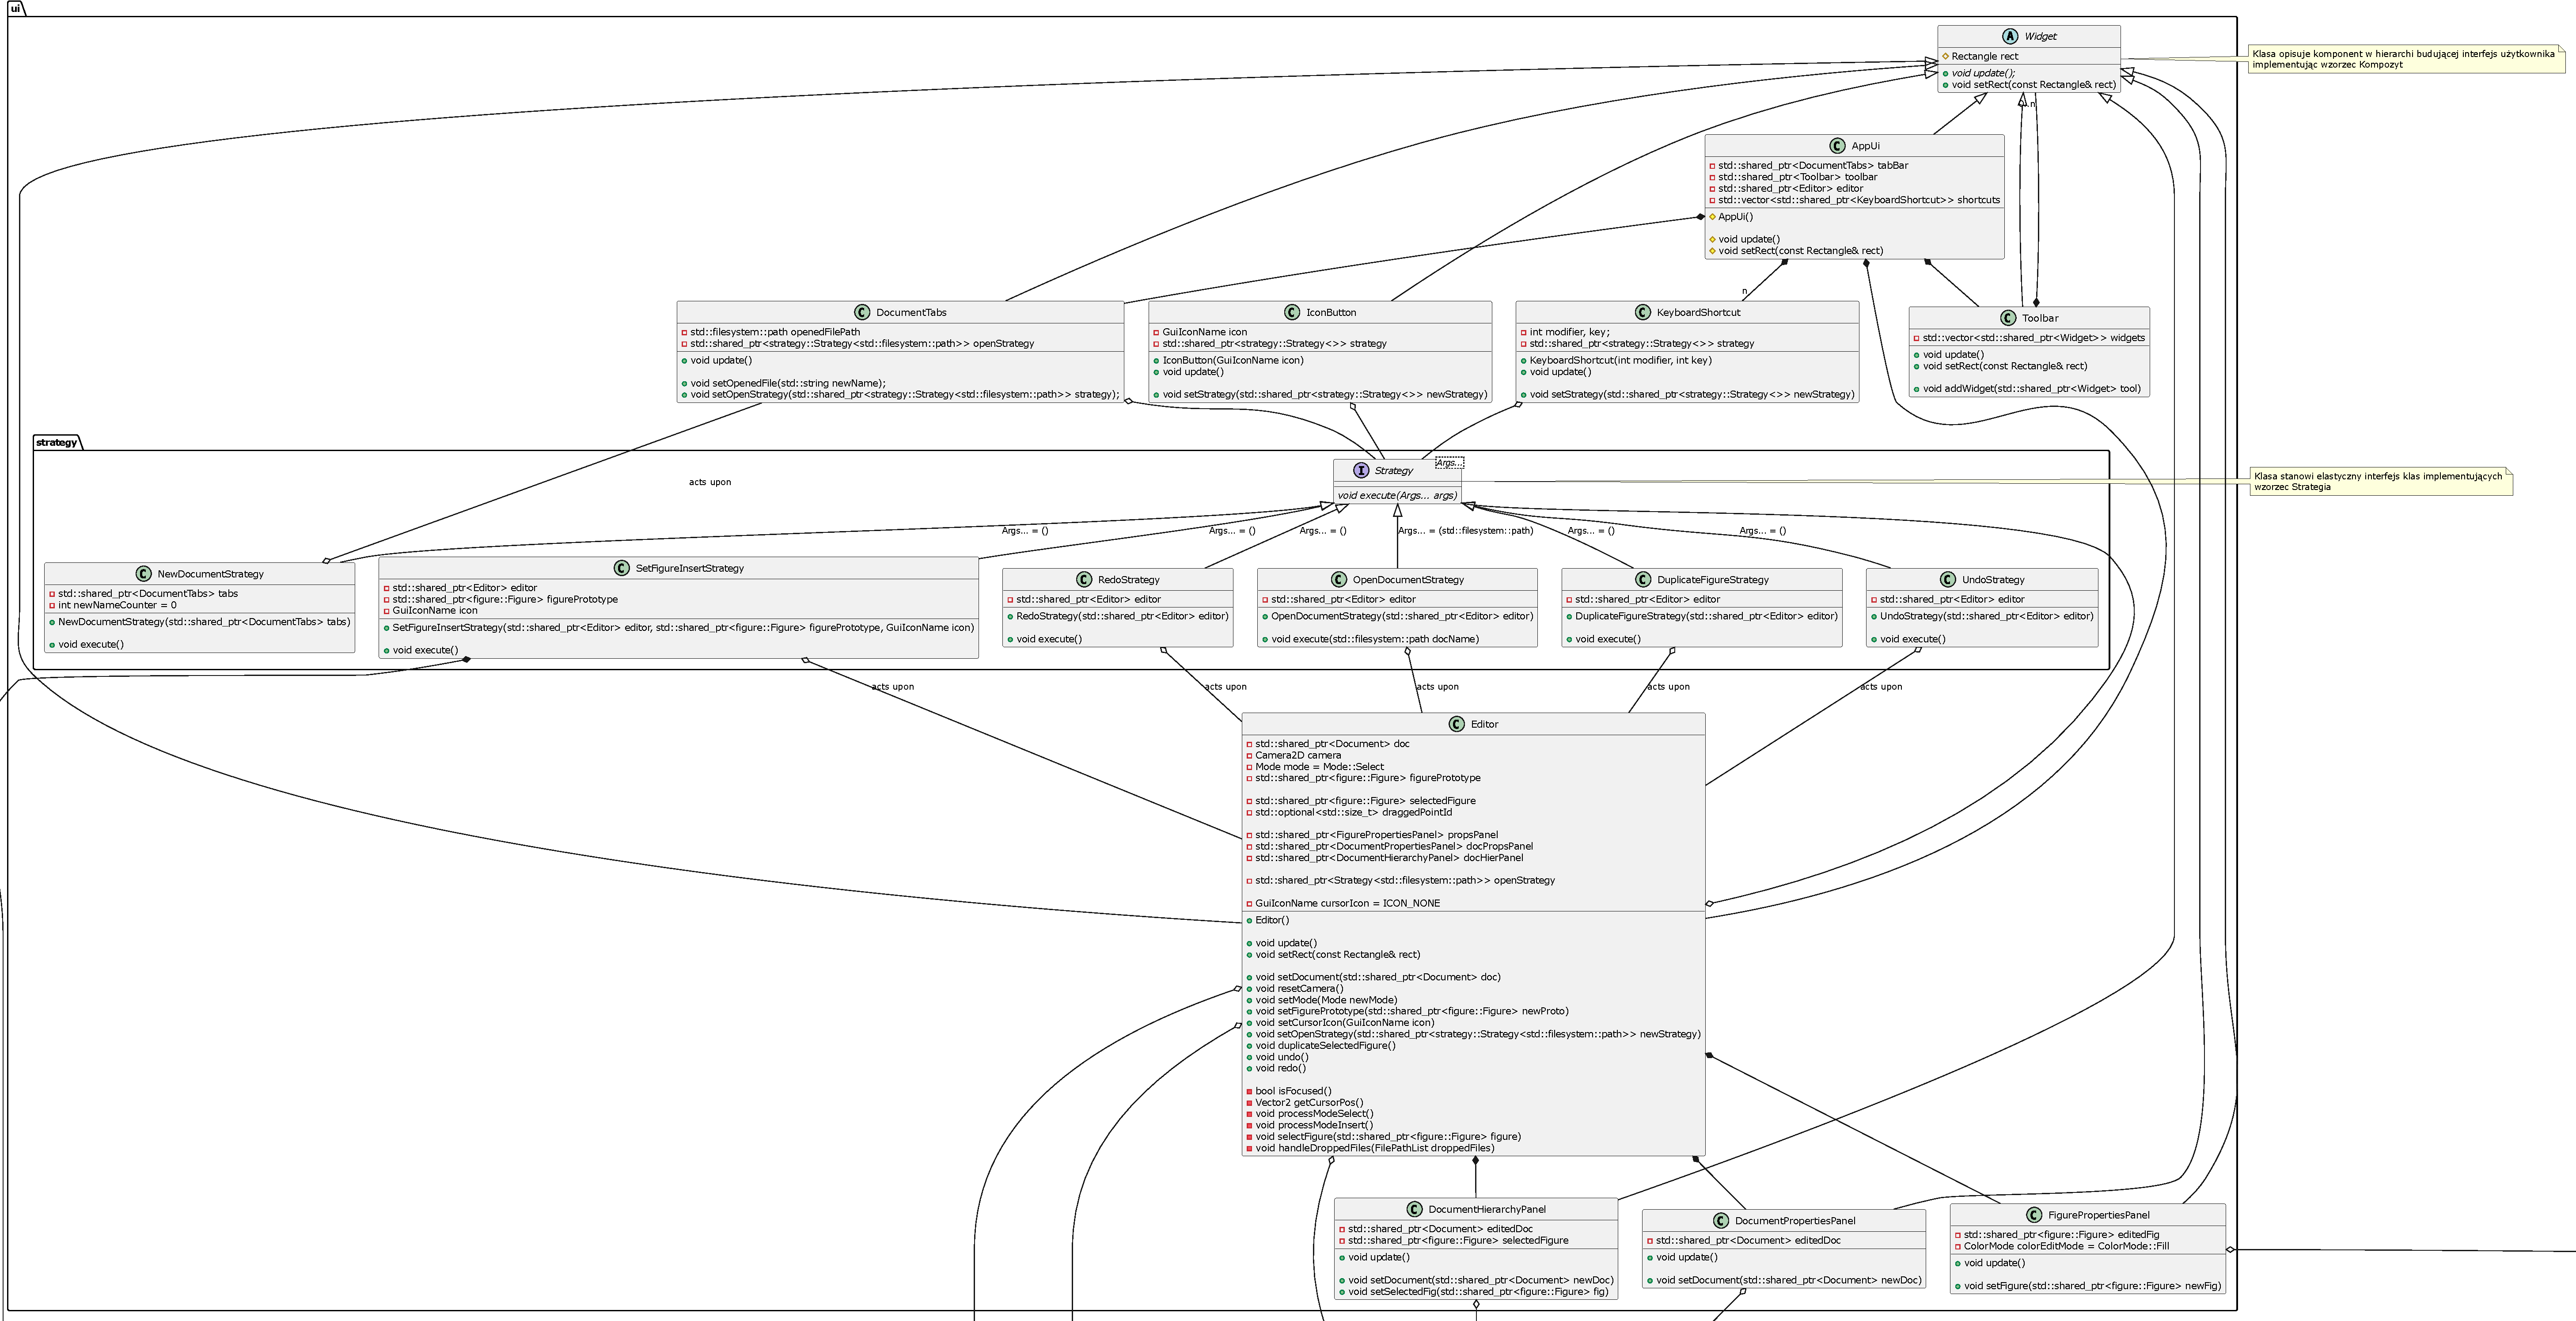
\includegraphics[width=0.7\textwidth]{figures/kompozyt.pdf}
	\end{figure}
\end{frame}

\begin{frame}
	\frametitle{Kompozyt - opis}
	Kompozyt to strukturalny wzorzec projektowy pozwalający komponować obiekty w struktury drzewiaste, a następnie traktować te struktury jakby były osobnymi obiektami.
	
	\vfill
	
	W naszym projekcie pozwala tworzyć hierarchię figur na grafice i w sposób rekurencyjny przetwarzać jej zawartość.
	
\end{frame}

\subsection{Metoda wytwórcza}

\begin{frame}
	\frametitle{Metoda wytwórcza}
	
	\begin{figure}
		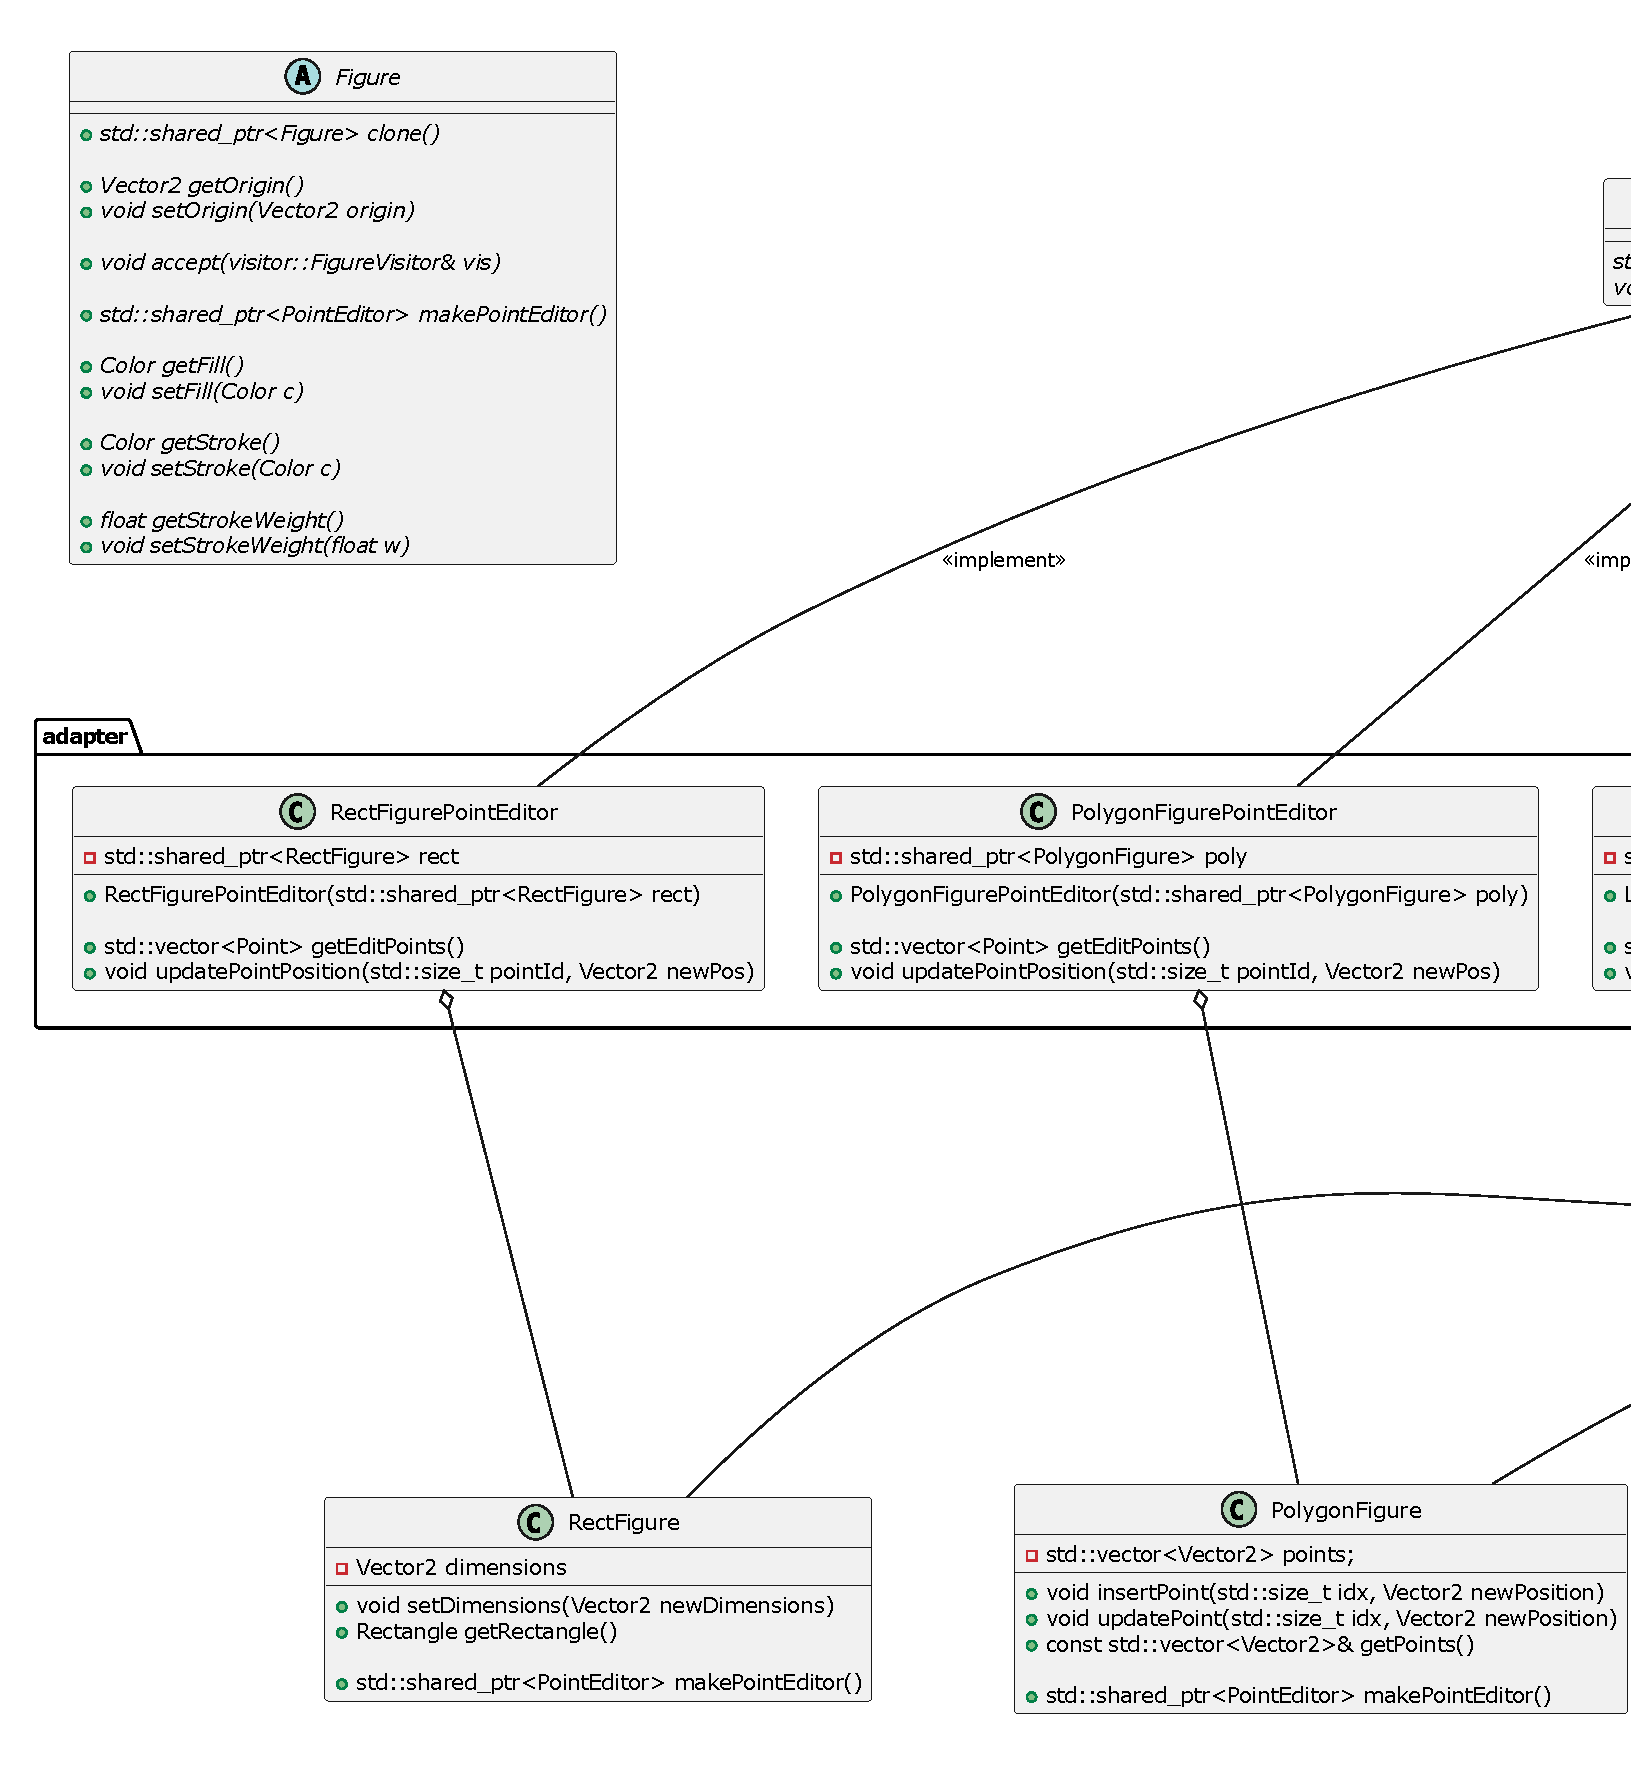
\includegraphics[height=0.7\textheight]{figures/fac.pdf}
	\end{figure}
\end{frame}

\begin{frame}
	\frametitle{Metoda wytwórcza - opis}
	Metoda wytwórcza jest kreacyjnym wzorcem projektowym, który udostępnia interfejs do tworzenia obiektów w ramach klasy bazowej, ale pozwala podklasom zmieniać typ tworzonych obiektów.
	
	\vfill
	
	W naszym projekcie metoda wytwórcza używana jest do tworzenia adapterów pozwalających na edycję konkretnych figur.
	
\end{frame}

\subsection{Strategia}

\begin{frame}
	\frametitle{Strategia}
	
	\begin{figure}
		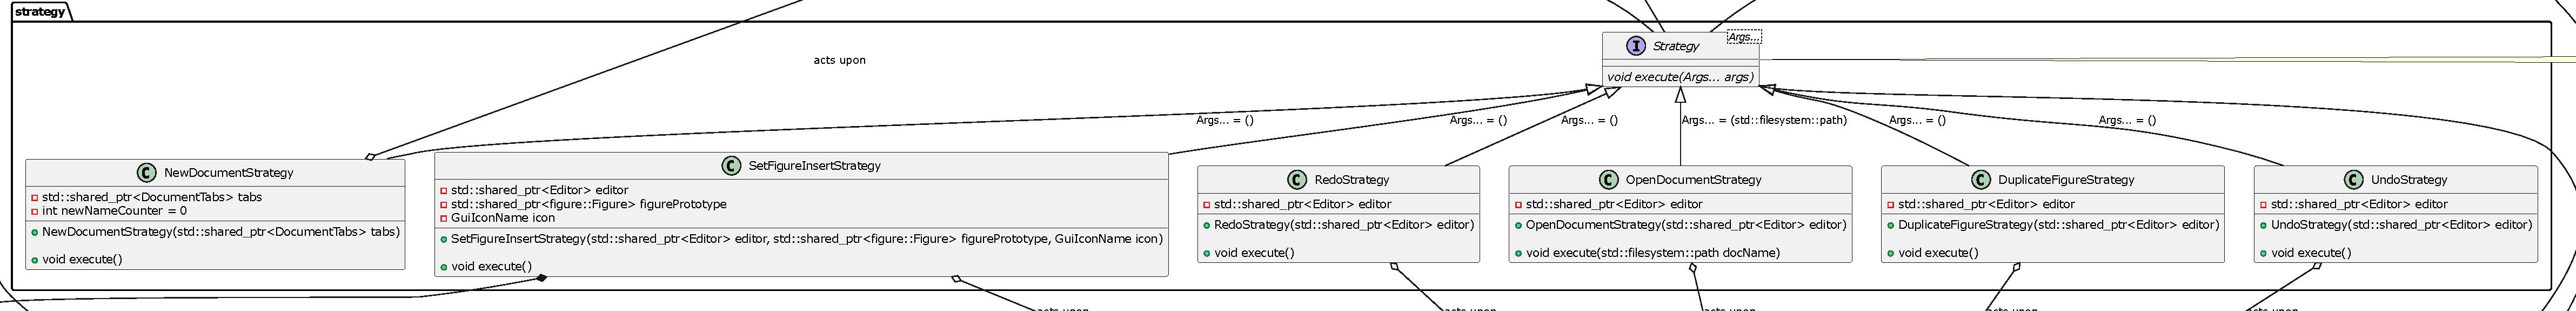
\includegraphics[width=0.9\textwidth]{figures/strategy.pdf}
	\end{figure}
\end{frame}

\begin{frame}
	\frametitle{Strategia - opis}
	Strategia to behawioralny wzorzec projektowy pozwalający zdefiniować rodzinę algorytmów, umieścić je w osobnych klasach i uczynić obiekty tych klas wymienialnymi.
	
	\vfill
	
	W naszym projekcie używamy jej do opisania akcji, które mają się wydarzyć w sytuacji kiedy użytkownik wciśnie guzik lub skorzysta ze skrótu klawiszowego.
	
\end{frame}

\subsection{Adapter}

\begin{frame}
	\frametitle{Adapter}
	
	\begin{figure}
		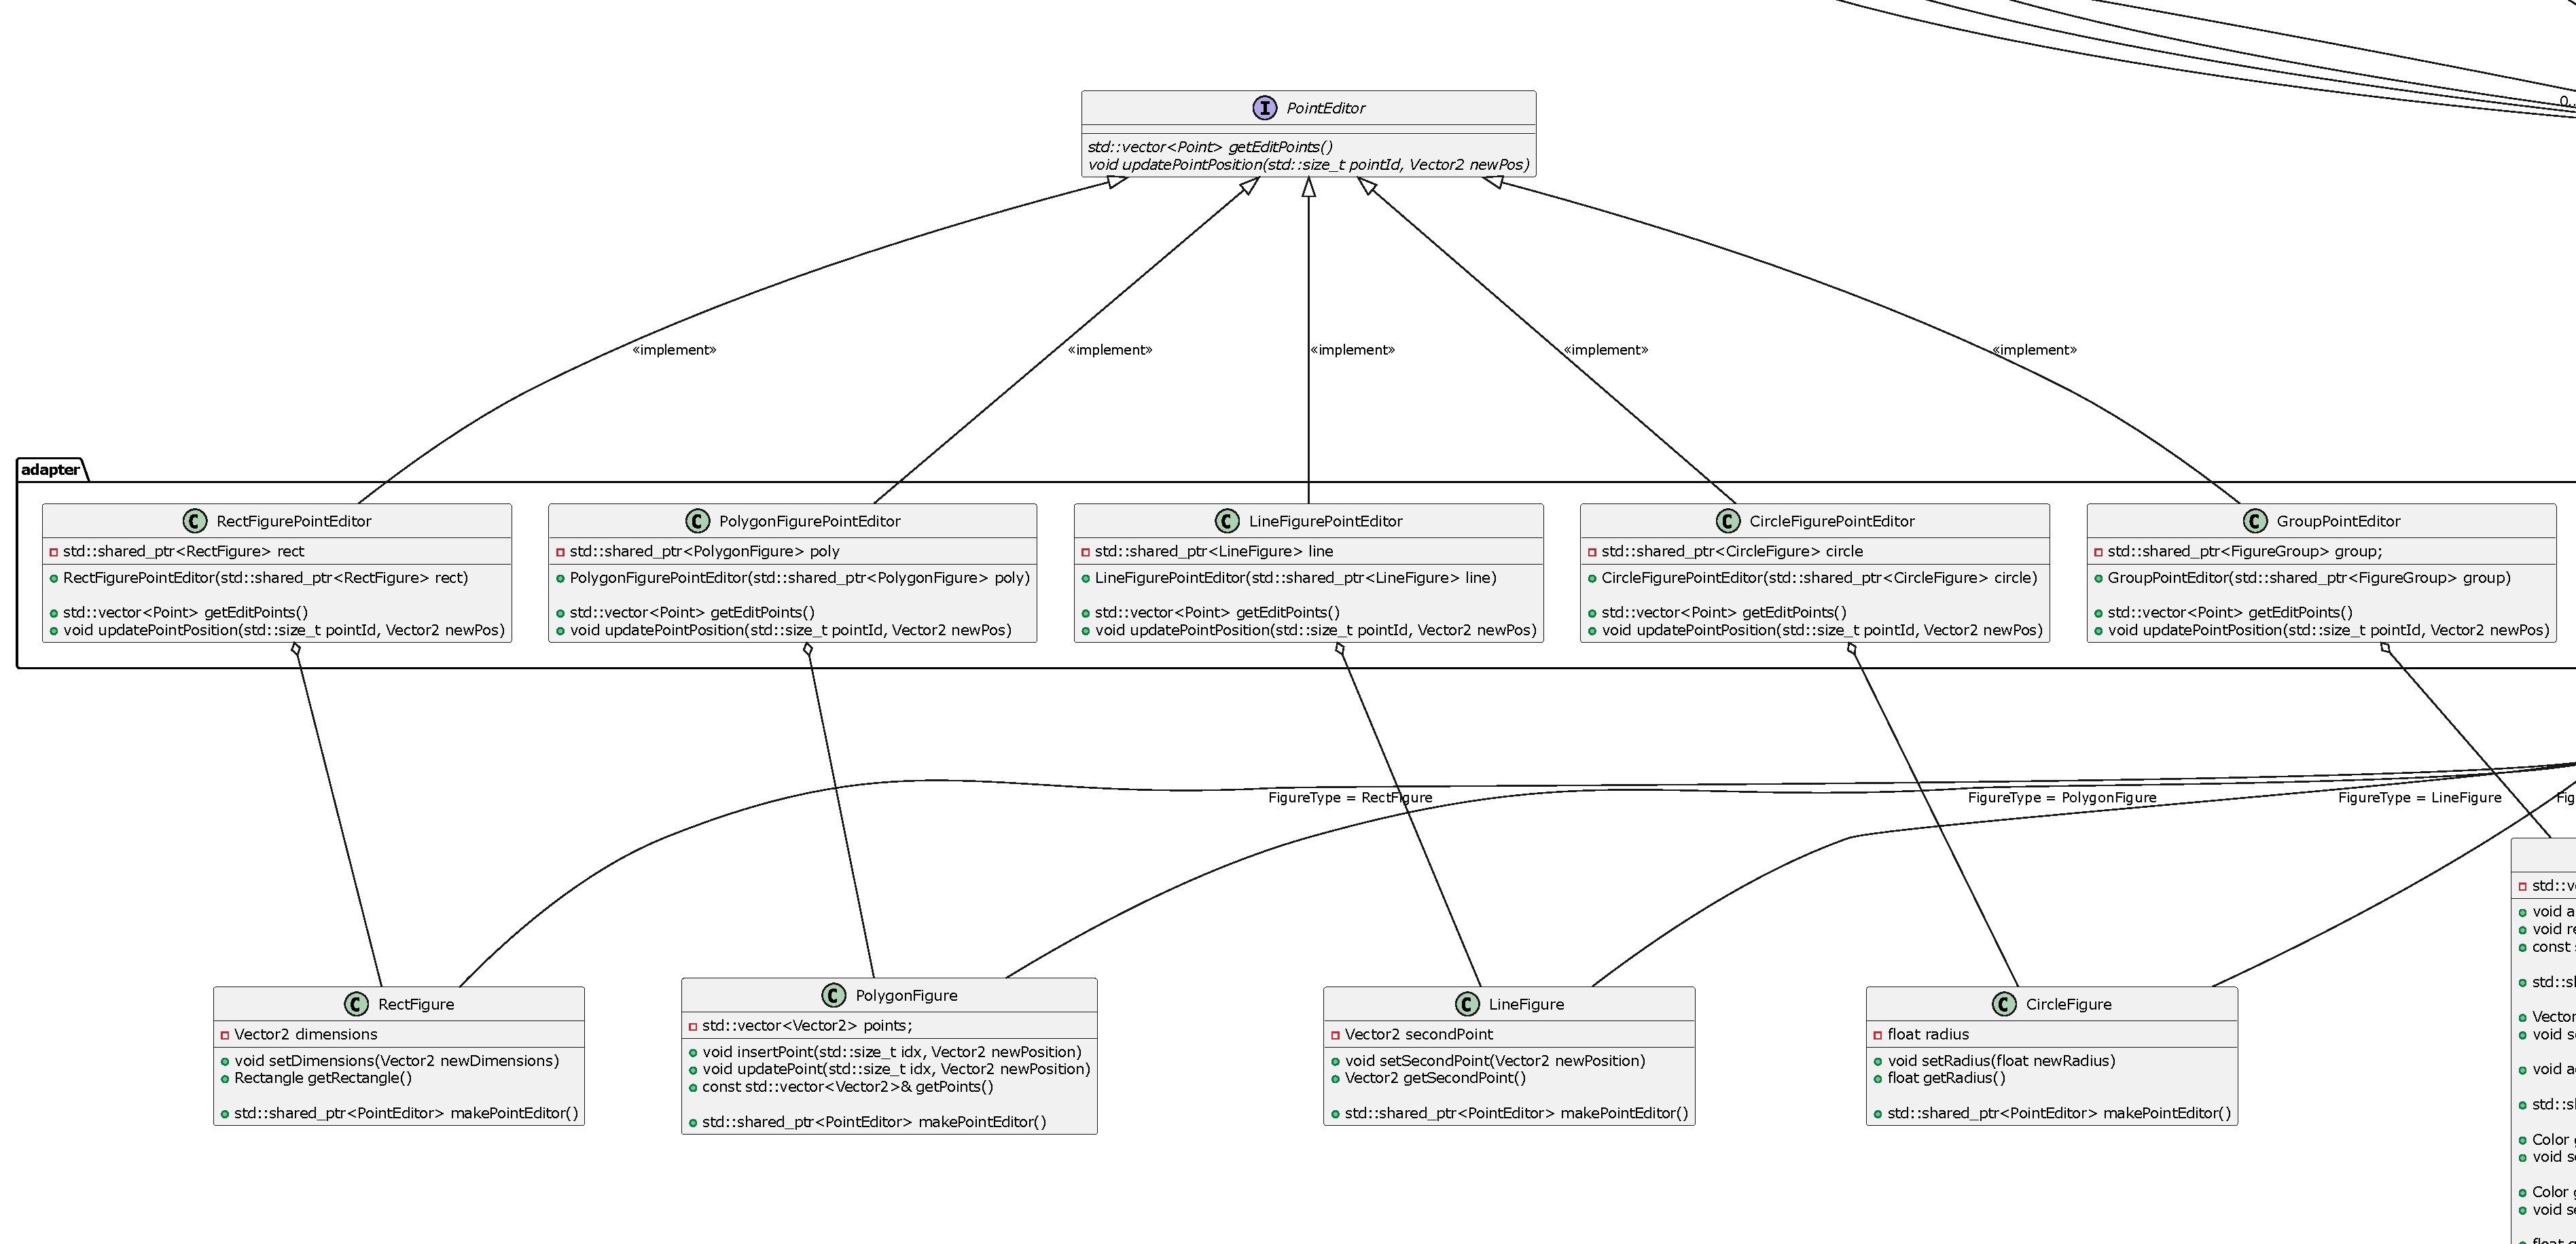
\includegraphics[width=0.9\textwidth]{figures/adapter.pdf}
	\end{figure}
\end{frame}

\begin{frame}
	\frametitle{Adapter - opis}
	Adapter jest strukturalnym wzorcem projektowym pozwalającym na współdziałanie ze sobą obiektów o niekompatybilnych interfejsach.
	
	\vfill
	
	W naszym projekcie tworzy wspólny interfejs do edytowania figur, które mogą posiadać różne własności i wielorakie sposoby ich edycji.
\end{frame}

\subsection{Odwiedzający}

\begin{frame}
	\frametitle{Odwiedzający}
	
	\begin{figure}
		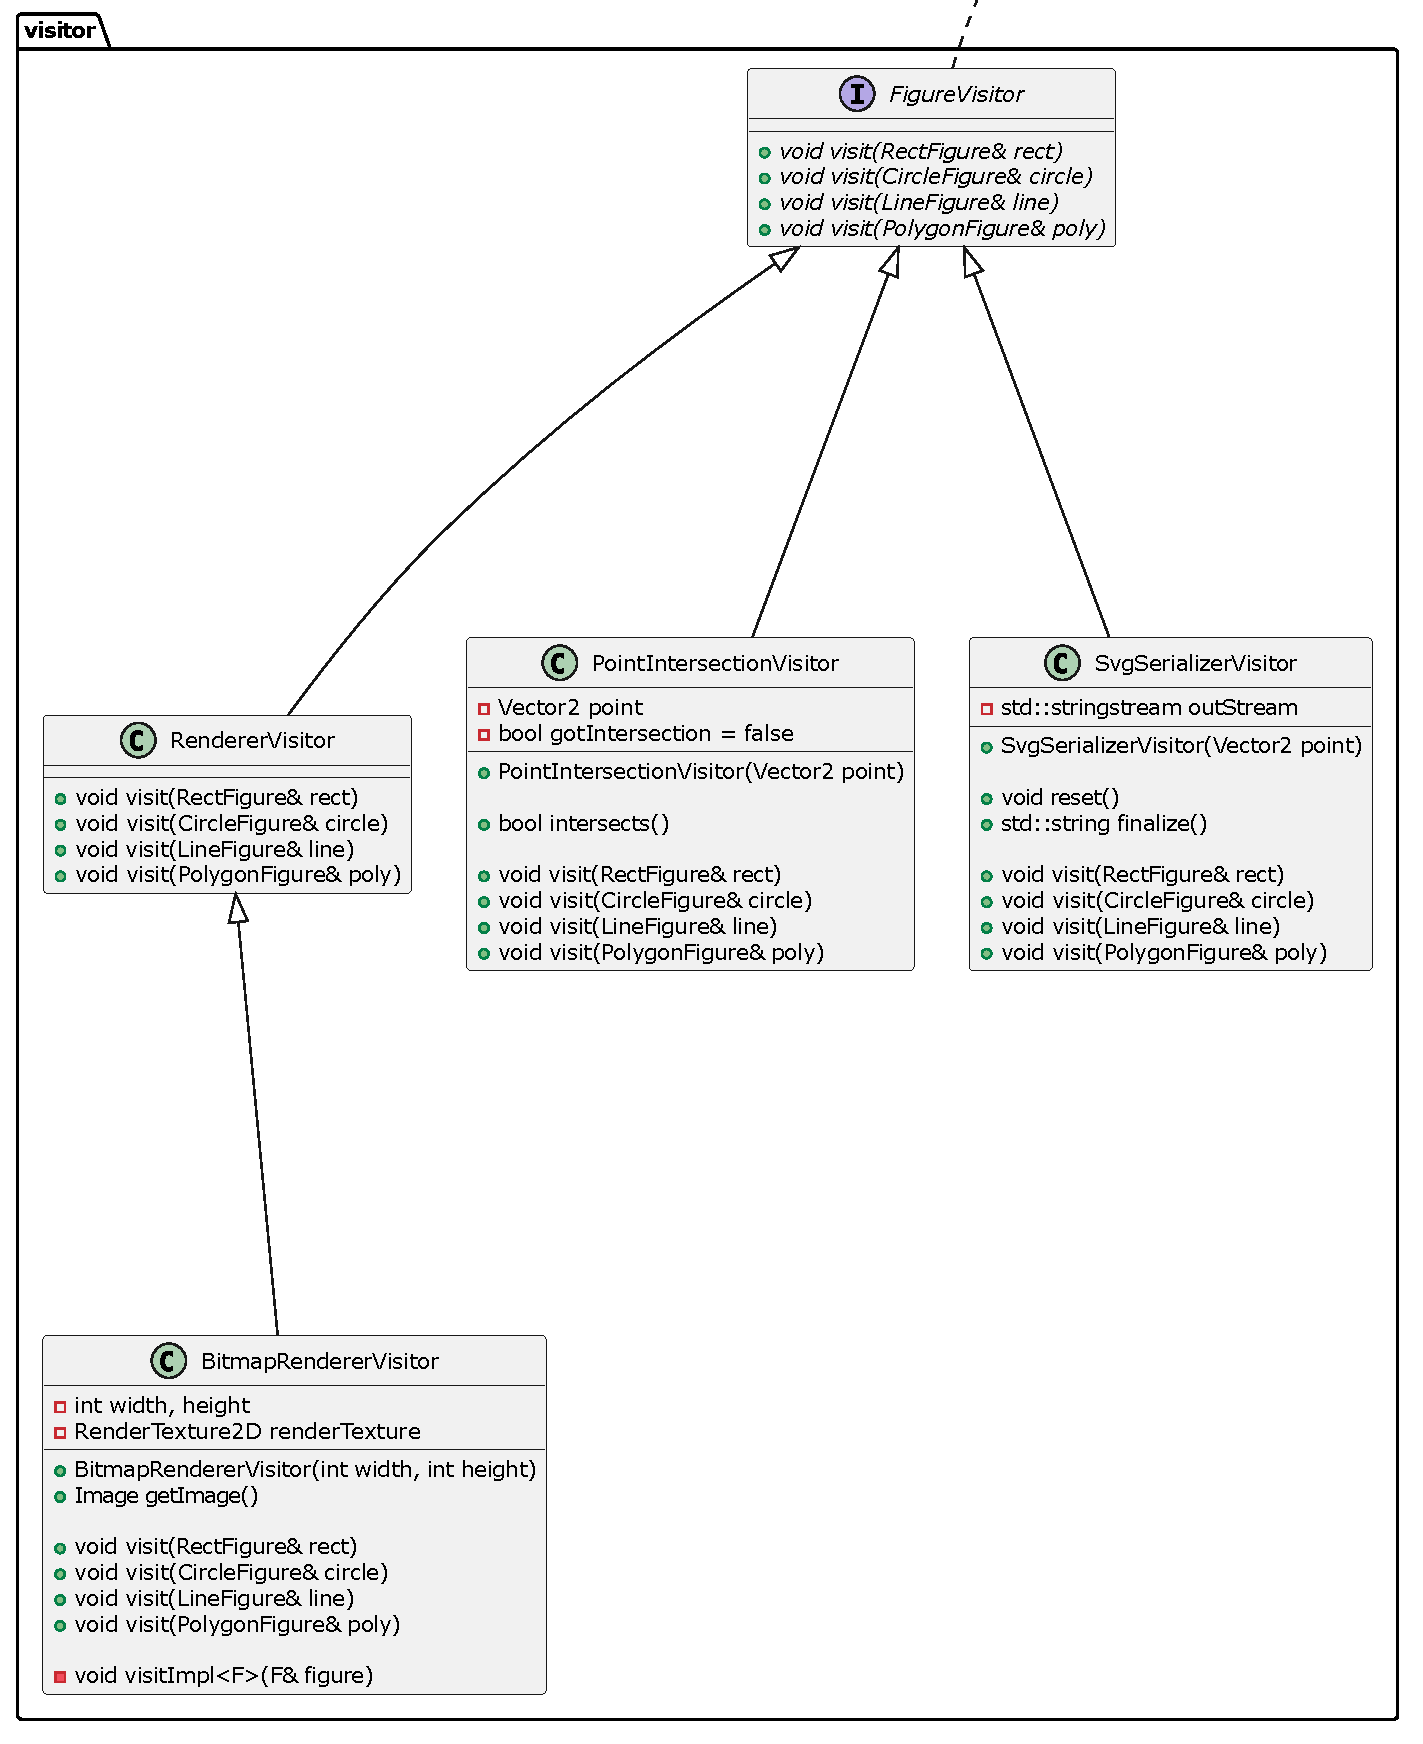
\includegraphics[height=0.7\textheight]{figures/visitor.pdf}
	\end{figure}
\end{frame}

\begin{frame}
	\frametitle{Odwiedzający}
	Odwiedzający to behawioralny wzorzec projektowy pozwalający oddzielić algorytmy od obiektów na których pracują.
	
	\vfill
	
	W naszym projekcie wzorzec jest użyty do rekurencyjnego przetwarzania figur z różnym sposobem obsługi we zależności od obsługi figury, Pozwala ograniczyć rolę klasy figury tylko do przechowania informacji o kształcie figury.
	
\end{frame}

\subsection{Prototyp}

\begin{frame}
	\frametitle{Prototyp}
	\begin{figure}
		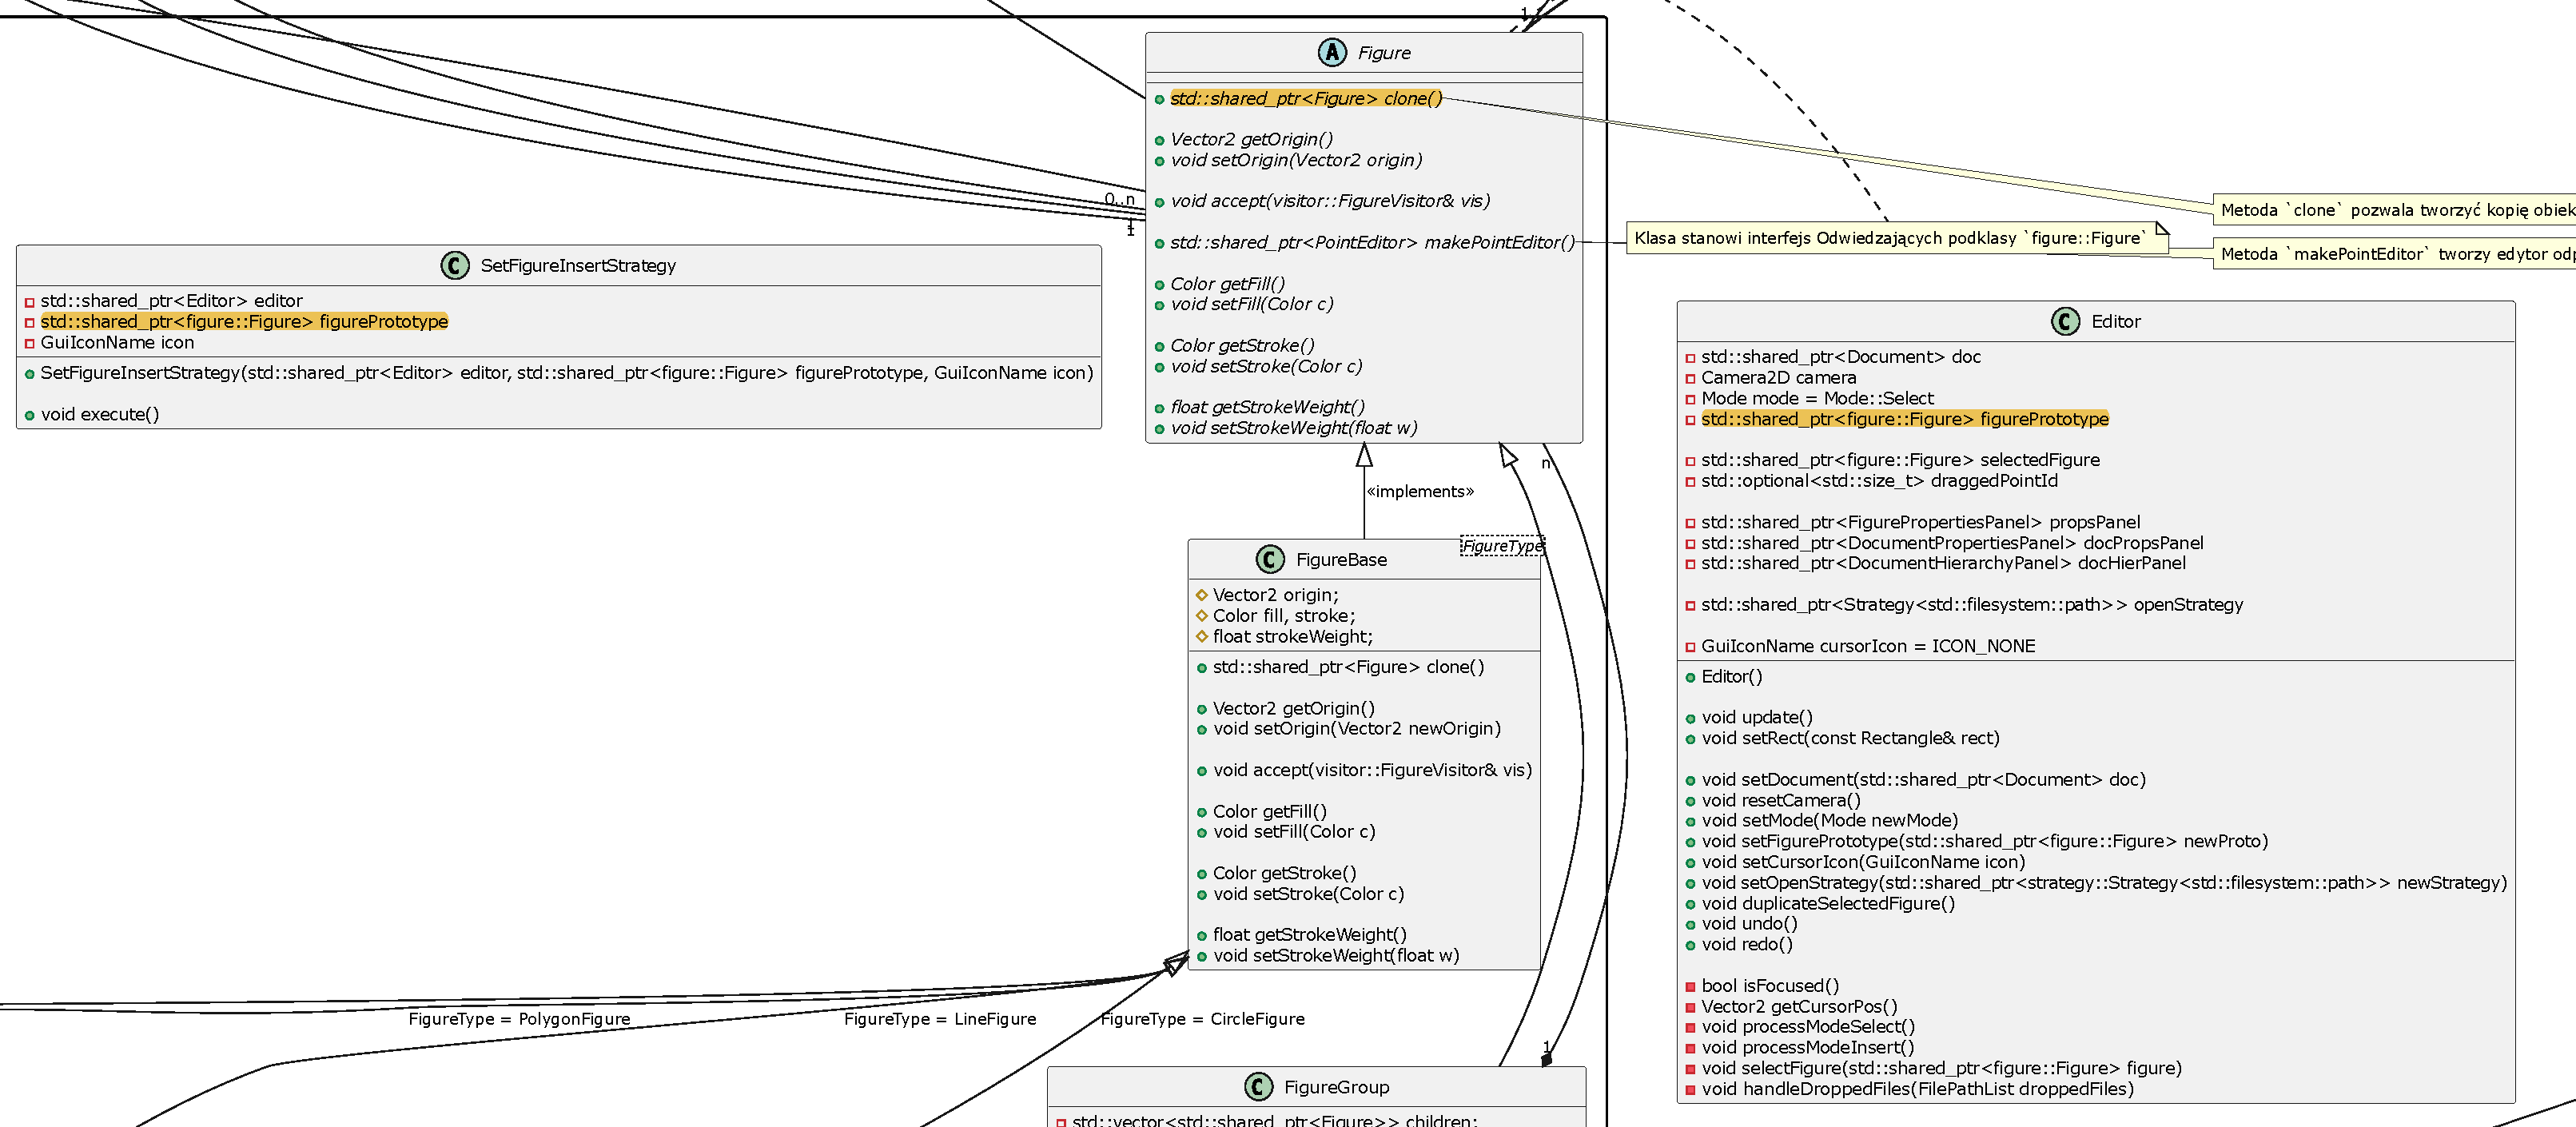
\includegraphics[width=0.7\textwidth]{figures/prototyp.pdf}
	\end{figure}
\end{frame}

\begin{frame}
	\frametitle{Prototyp - opis}
	Prototyp to kreacyjny wzorzec projektowy, który umożliwia kopiowanie już istniejących obiektów bez tworzenia zależności pomiędzy twoim kodem, a klasami obiektów.
	
	\vfill
	
	W naszym projekcie prototyp pozwala na tworzenie nowych figur w oparciu o zdefiniowane wzorcowe figury
\end{frame}

%------------------------------------------------

\section{Początkowa implementacja}

\begin{frame}
	\frametitle{Początkowa implementacja}
	\framesubtitle{Ekran startowy}
	
	\begin{figure}
		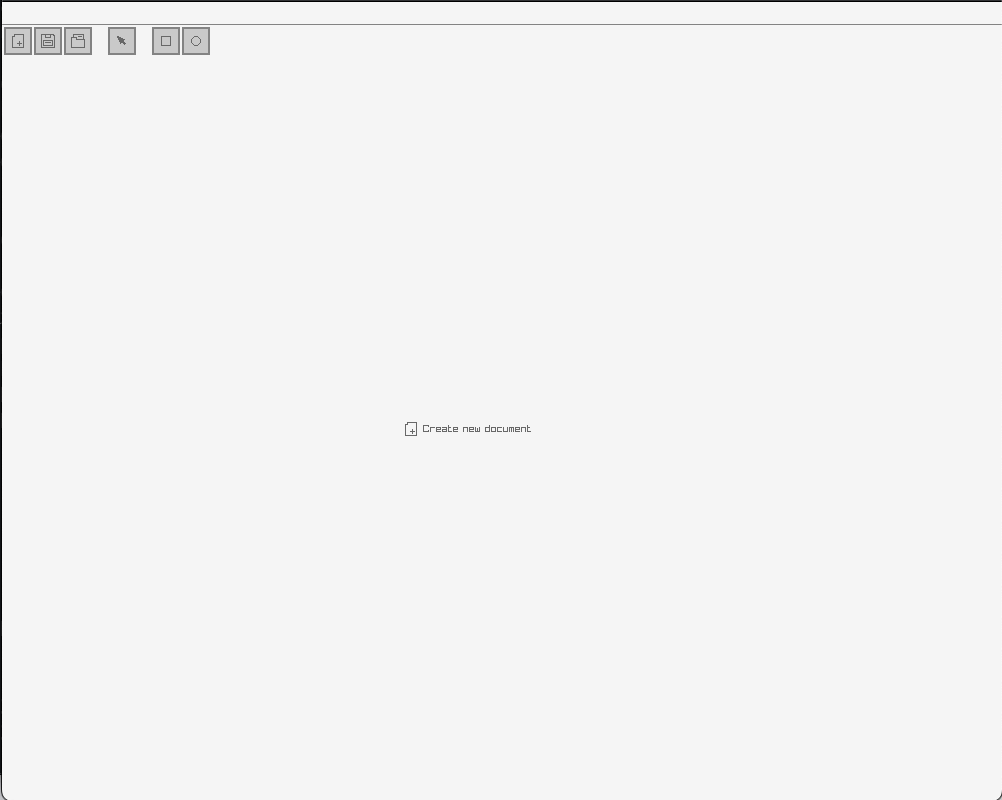
\includegraphics[height=0.7\textheight]{figures/pro1.png}
	\end{figure}
\end{frame}

\begin{frame}
	\frametitle{Początkowa implementacja}
	\framesubtitle{Tworzenie pliku}
	
	\begin{figure}
		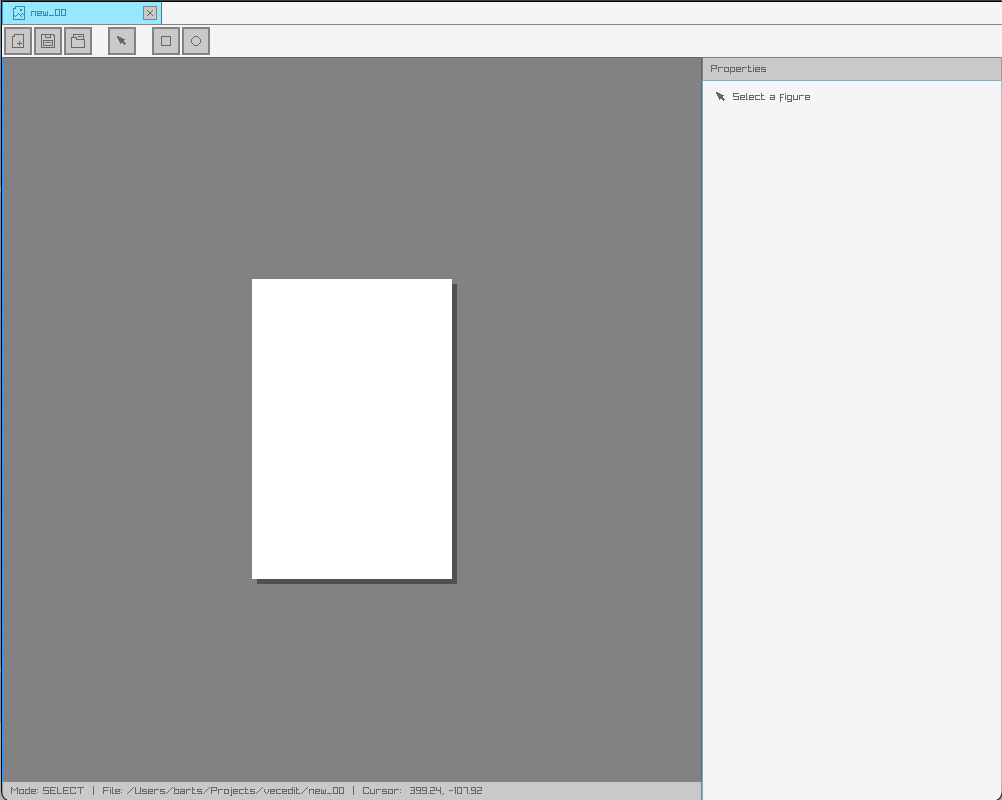
\includegraphics[height=0.7\textheight]{figures/pro2.png}
	\end{figure}
\end{frame}

\begin{frame}
	\frametitle{Początkowa implementacja}
	\framesubtitle{Dodanie figury}
	
	\begin{figure}
		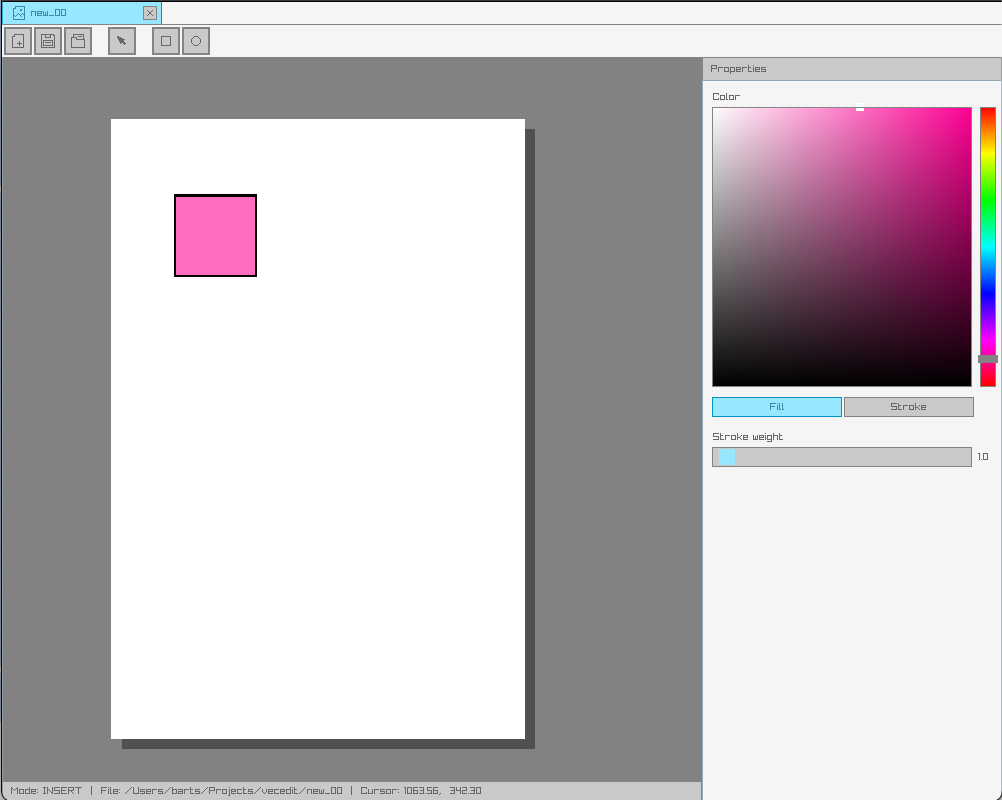
\includegraphics[height=0.7\textheight]{figures/pro3.png}
	\end{figure}
\end{frame}

\begin{frame}
	\frametitle{Początkowa implementacja}
	\framesubtitle{Edycja figury}
	
	\begin{figure}
		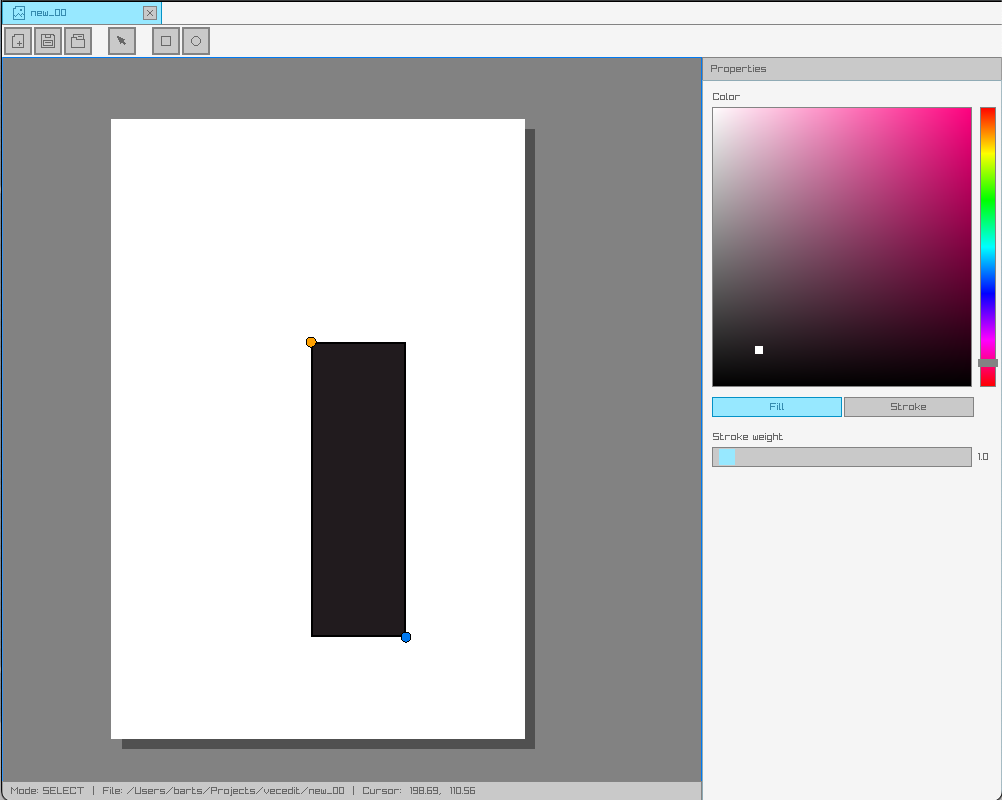
\includegraphics[height=0.7\textheight]{figures/pro4.png}
	\end{figure}
\end{frame}

\begin{frame}
	\frametitle{Początkowa implementacja}
	\framesubtitle{Dodanie kolejnej figury}
	
	\begin{figure}
		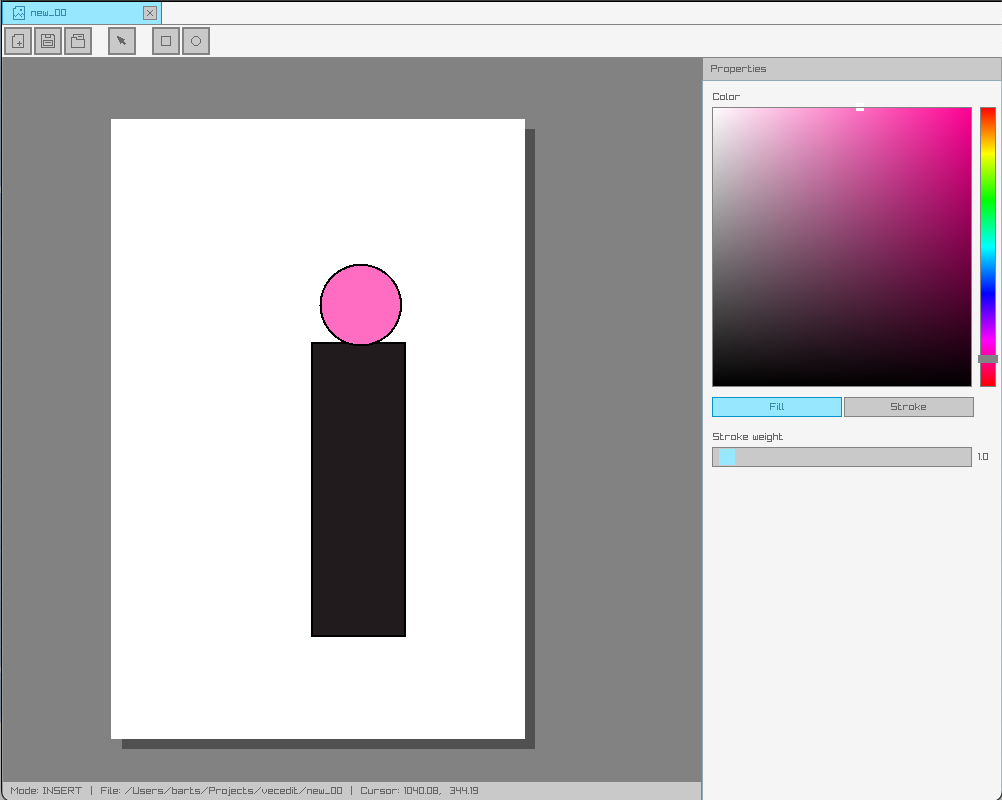
\includegraphics[height=0.7\textheight]{figures/pro5.png}
	\end{figure}
\end{frame}

\begin{frame}
	\frametitle{Początkowa implementacja}
	\framesubtitle{Nakładanie się figur}
	
	\begin{figure}
		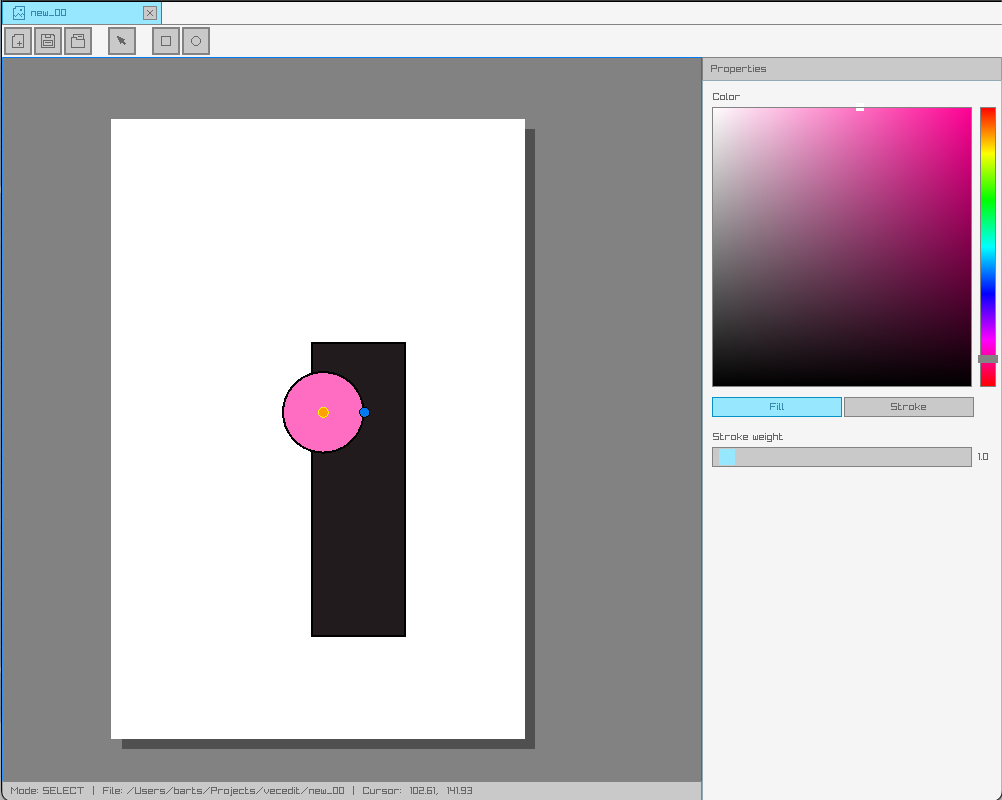
\includegraphics[height=0.7\textheight]{figures/pro6.png}
	\end{figure}
\end{frame}

\begin{frame}
	\frametitle{Początkowa implementacja}
	\framesubtitle{Zmiany parametrów figur}
	
	\begin{figure}
		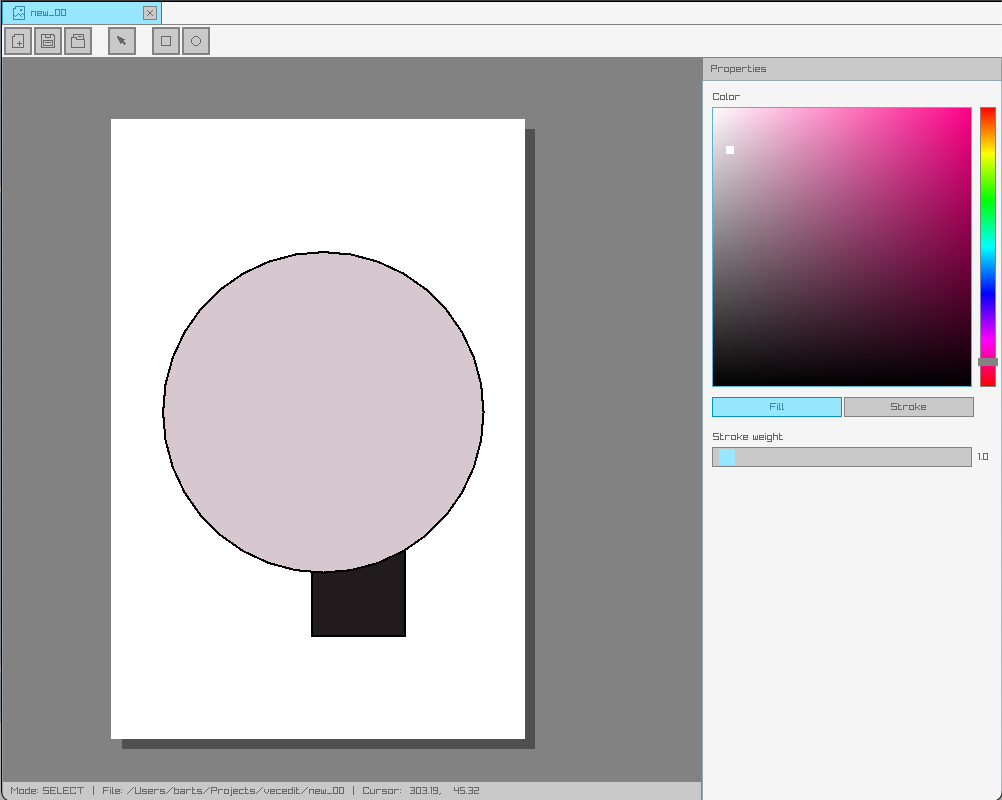
\includegraphics[height=0.7\textheight]{figures/pro7.png}
	\end{figure}
\end{frame}

\begin{frame}
	\frametitle{Początkowa implementacja}
	\framesubtitle{Zmiany parametrów figur}
	
	\begin{figure}
		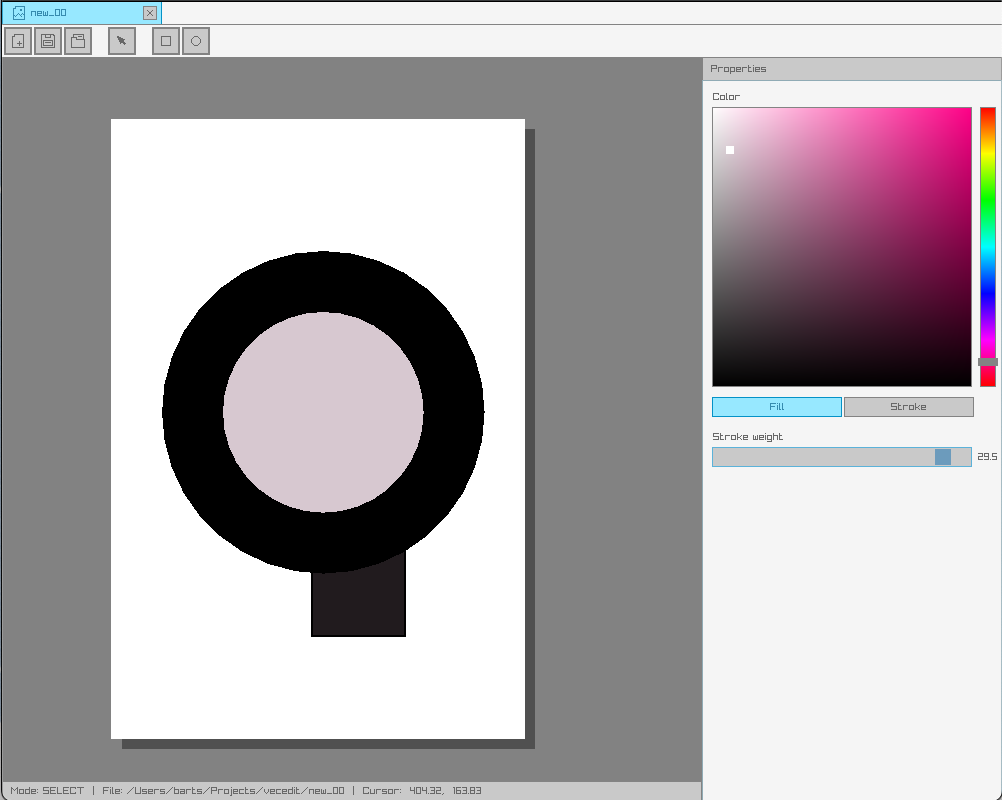
\includegraphics[height=0.7\textheight]{figures/pro8.png}
	\end{figure}
\end{frame}

\begin{frame}
	\frametitle{Początkowa implementacja}
	\framesubtitle{Zmiany parametrów figur}
	
	\begin{figure}
		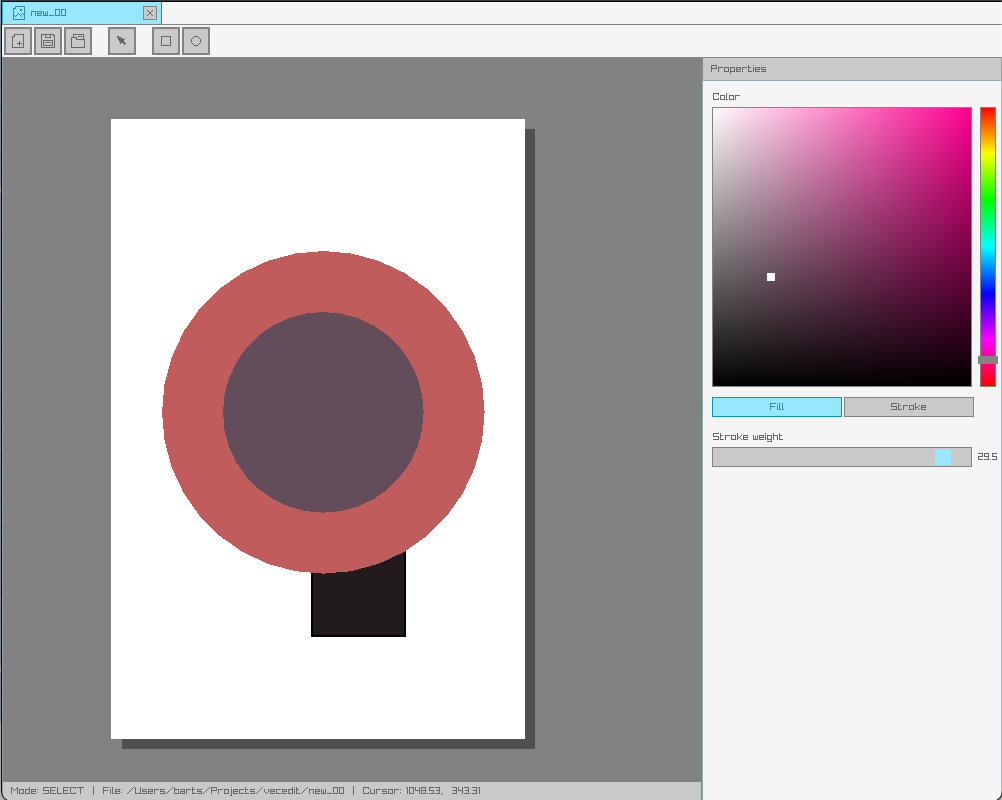
\includegraphics[height=0.7\textheight]{figures/pro9.png}
	\end{figure}
\end{frame}
%------------------------------------------------


%----------------------------------------------------------------------------------------
%	CLOSING SLIDE
%----------------------------------------------------------------------------------------

\begin{frame}[plain] % The optional argument 'plain' hides the headline and footline
	\begin{center}
		{\Huge Koniec}
		
		\bigskip\bigskip % Vertical whitespace
		
		{\LARGE Dziękujemy za uwagę}
	\end{center}
\end{frame}

%----------------------------------------------------------------------------------------

\end{document} 
